% Provenance (never printed): see sources/outline_sources.md (Year 1: morphology,
% gravity, heat flow and seismicity of a subduction zone; accretionary and erosive
% margins; slab geometry; volcanic arcs). Kuril map, section and numbers from
% figdata/bachelor-1/slab_seismicity.py; exercise and problem values in the Book 3
% scratch calculator calc/ch14.py.
\chapter{Márgenes activos}\label{ch:b1:active-margins}

El 11 de marzo de 2011, a las 14:46 hora local, la frontera de placas frente al noreste de Japón se rompió a lo largo de unos
\qty{400}{km} de la fosa y \qty{150}{km} hacia abajo de su \omterm{def:b1:geological-maps:attitude}{buzamiento}. La falla se deslizó de 50 a \qty{60}{m}, sobre todo por encima del
hipocentro, hacia la fosa de Japón; en tierra, la costa se movió horizontalmente y se hundió. La placa que se hunde allí, la placa del
Pacífico, desciende bajo Japón a lo largo de un plano que los terremotos dibujan hasta cientos de kilómetros de profundidad; y donde ese
plano yace a unos cien kilómetros de profundidad, una línea de volcanes corre paralela a la costa. Este capítulo lee un margen así a partir
de su forma, su gravedad, su \omterm{def:b1:heat-budget:heat-flow}{flujo de calor} y, sobre todo, sus terremotos.
% ledger: usgs:tohoku, wada:decoupling

\begin{recall}
La \omterm{def:b1:layered-earth:lithosphere}{litosfera} oceánica se hunde de nuevo en el \omterm{def:b1:layered-earth:layers}{manto} en las zonas de subducción, marcadas por fosas y por zonas inclinadas de terremotos, y la
\omterm{def:b1:layered-earth:lithosphere}{litosfera} vieja se hunde bajo su propio peso (libro 2, año 11); el agua de la placa que se hunde baja la temperatura de fusión del \omterm{def:b1:layered-earth:layers}{manto} que
hay encima (libro 2, año 12). El calor se difunde a lo largo de una distancia $L$ en un tiempo del orden de $L^2/\kappa$
(\cref{ch:b1:heat-budget}); una placa infinita de densidad $\rho$ y espesor $h$ atrae con $2\pi G\rho h$ (\cref{ch:b1:isostasy-gravity});
las placas se mueven alrededor de \omterm{def:b1:plate-kinematics:euler-pole}{polos de Euler} (\cref{ch:b1:plate-kinematics}); el \omterm{def:b1:heat-budget:heat-flow}{flujo de calor} del fondo oceánico decae como la raíz
cuadrada inversa de su edad (\cref{ch:b1:rifts-ridges-margins}).
\end{recall}

\section{La anatomía de un margen activo}\label{sec:b1:active-margins:anatomy}

\begin{definition}[Margen activo, fosa oceánica, antearco, cuenca de tras-arco]\label{def:b1:active-margins:active-margin}
Un \emph{margen activo}\index{margen activo} es una frontera de placas convergente en la que la \omterm{def:b1:layered-earth:lithosphere}{litosfera} oceánica se hunde bajo otra placa,
bajo un continente o bajo otra placa oceánica. Una \emph{fosa oceánica}\index{fosa oceánica} es la depresión larga, estrecha y en forma de V
del fondo marino a lo largo de la cual la placa que se hunde se curva hacia abajo bajo la otra. El \emph{antearco}\index{antearco} es la parte
de la placa cabalgante entre la fosa y la línea de volcanes. Una \emph{cuenca de tras-arco}\index{cuenca de tras-arco} es una cuenca detrás de
los volcanes, en el lado alejado de la fosa, donde la placa cabalgante se estira y puede formarse \omterm{def:b1:rifts-ridges-margins:oceanic-crust}{corteza oceánica} nueva.
\end{definition}

Las fosas son los lugares más profundos de los océanos, y el más profundo de todos es el Abismo Challenger de la fosa de las Marianas. A
través de la fosa de las Kuriles el fondo desciende desde unos \qty{5200}{m} en la llanura abisal hasta \qty{8700}{m} en el eje, unos
\qty{3.5}{km} más bajo, y la fosa tiene solo decenas de kilómetros de anchura (figura en \cref{sec:b1:active-margins:gravity-heat}). Los
márgenes convergentes de la Tierra miden unos \qty{55000}{km} en total; en un modelo digital de las fronteras de placas, las fronteras de
subducción suman unos \qty{51000}{km}, frente a unos \qty{67000}{km} de dorsales de expansión.
% ledger: data:b3-grav-kuril (trench_gravity.py values), stern:subduction, data:pb2002 (ridge_budget.py)

Por delante de la fosa, la placa se eleva ligeramente antes de hundirse, en una elevación exterior amplia y baja. Allí la placa está curvada,
y su parte superior está estirada: los terremotos de fallamiento normal se producen en las elevaciones exteriores. La anchura de la elevación
exterior coincide con la flexión de una placa elástica; esta flexión de la \omterm{def:b1:layered-earth:lithosphere}{litosfera} se estudia en el libro de tercer año universitario. La
propia fosa es el lugar donde el peso de la placa densa que se hunde tira de su borde delantero hacia abajo.

\begin{definition}[Losa en subducción]\label{def:b1:active-margins:slab}
La \emph{losa en subducción}\index{losa en subducción} es la parte de la placa que se hunde que ya ha descendido al \omterm{def:b1:layered-earth:layers}{manto}: una lámina de
\omterm{def:b1:layered-earth:lithosphere}{litosfera} oceánica, con su \omterm{def:b1:layered-earth:layers}{corteza} encima, inclinada bajo la placa cabalgante desde la fosa hasta profundidades de varios cientos de kilómetros.
\end{definition}

La placa cabalgante se corta en franjas paralelas a la fosa (figura de abajo): el \omterm{def:b1:active-margins:active-margin}{antearco}, a menudo con una pila de sedimentos raspados en su
frente y una cuenca sedimentaria detrás; el \omterm{def:b1:active-margins:volcanic-arc}{arco volcánico}; y, detrás de algunos arcos, una \omterm{def:b1:active-margins:active-margin}{cuenca de tras-arco} y un arco antiguo y extinguido
más allá. Entre la losa y la placa cabalgante yace una cuña de \omterm{def:b1:layered-earth:layers}{manto}, arrastrada hacia abajo a lo largo de la cima de la losa.

\begin{omfigure}
\begin{tikzpicture}[x=0.01667cm, y=0.01667cm, font=\scriptsize,
  lbl/.style={fill=white, fill opacity=0.8, text opacity=1, inner sep=1pt}]
\begin{scope}
\clip (-150,-330) rectangle (650,55);
% mantle and sea water
\fill[orange!12] (-150,-330) rectangle (650,15);
\fill[omSea!45] (-150,15) rectangle (650,0);
% incoming plate and slab: top dips 25 deg to 50 km, then 45 deg; 100 km thick
\fill[omLithBasalt!55] (-150,4) -- (-80,4) .. controls (-60,7) and (-40,7) .. (-25,4) -- (0,0)
  -- (107.2,-50) -- (420,-363) -- (349,-434) -- (48.9,-133.1) -- (-22.1,-100) -- (-150,-100) -- cycle;
\draw[omSea!50!black, line width=1.6pt] (-150,4) -- (-80,4) .. controls (-60,7) and (-40,7) .. (-25,4) -- (0,0) -- (107.2,-50) -- (420,-363);
% overriding plate
\fill[brown!28] (0,0) -- (12,3) -- (45,8) -- (60,10) -- (140,10) -- (150,12) -- (184,12) -- (230,9)
  -- (300,7) -- (395,6) -- (410,3) -- (420,2) -- (430,3) -- (445,6) -- (540,7) -- (560,14) -- (590,14)
  -- (610,10) -- (650,10) -- (650,-60) -- (520,-55) -- (445,-25) -- (420,-15) -- (395,-25) -- (320,-55)
  -- (250,-60) -- (117.2,-60) -- (107.2,-50) -- cycle;
% accretionary prism and forearc basin
\fill[yellow!55] (0,0) -- (12,3) -- (45,8) -- (60,10) -- (60,-28) -- cycle;
\draw[black!45, line width=0.3pt] (14,-3) -- (24,5) (28,-7) -- (38,6) (42,-14) -- (52,8);
\fill[yellow!30] (68,10) -- (132,10) -- (122,4) -- (78,4) -- cycle;
% arc volcano
\fill[black!60] (150,12) -- (167,26) -- (184,12) -- cycle;
% an isotherm: a cold tongue down the slab
\draw[omDef, dashed, line width=0.6pt] (-150,-82) -- (-30,-82) -- (40,-118) -- (300,-318)
  -- (232,-200) -- (150,-112) .. controls (130,-80) and (180,-72) .. (260,-72) -- (650,-72);
% mantle wedge flow
\draw[->, black!60, line width=0.5pt] (600,-130) .. controls (450,-135) and (300,-125) .. (215,-150)
  .. controls (205,-160) and (240,-185) .. (300,-235);
% water and melt
\foreach \x/\z in {150/-93, 172/-115, 194/-137}
  \draw[->, blue!70!black, line width=0.5pt] (\x,\z) -- (\x-6,\z+28);
\draw[red!75!black, line width=0.8pt, decorate, decoration={snake, amplitude=1.2, segment length=6}] (167,-100) -- (167,12);
% earthquakes
\foreach \x/\z in {20/-12, 45/-22, 70/-34, 95/-45, 60/-40, 85/-58, 120/-70, 135/-85, 150/-104,
  165/-112, 185/-140, 205/-150, 225/-175, 248/-195, 270/-216, 290/-242, 312/-262, 330/-282, 350/-300, 365/-318}
  \fill[black] (\x,\z) circle[radius=0.9pt];
% the 100-km level beneath the arc
\draw[black!70, densely dotted] (90,-100) -- (260,-100);
\draw[black!70, densely dotted] (167,12) -- (167,-110);
\end{scope}
\draw[black!70] (-150,-330) rectangle (650,55);
\node[lbl, anchor=south] at (-85,15) {elevación exterior};
\node[lbl, anchor=south] at (0,15) {fosa};
\node[lbl, anchor=west] (pr) at (75,-28) {prisma de acreción};
\draw[black!70] (pr.west) -- (38,-6);
\node[lbl, anchor=south] at (88,15) {antearco};
\node[lbl, anchor=south] at (185,27) {arco volcánico};
\node[lbl, anchor=south] at (420,15) {cuenca de tras-arco};
\node[lbl, anchor=south] at (575,15) {arco remanente};
\node[lbl, anchor=west] at (-140,-50) {litosfera oceánica};
\node[lbl, anchor=east] (sl) at (120,-262) {losa en subducción};
\draw[black!70] (sl.east) -- (205,-262);
\node[lbl, anchor=west] (wb) at (420,-265) {zona de Wadati--Benioff};
\draw[black!70] (wb.west) -- (318,-266);
\node[lbl] at (430,-170) {cuña del manto};
\node[lbl] at (575,-30) {placa cabalgante};
\node[lbl, anchor=west, text=blue!70!black] at (212,-98) {agua};
\node[lbl, anchor=east] at (88,-100) {\qty{100}{km} de profundidad};
\node[lbl, anchor=west, text=omDef] at (450,-95) {una isoterma};
\node[lbl, anchor=west] at (-140,-300) {manto};
\draw[line width=1pt] (500,-310) -- (600,-310) node[midway, above] {\qty{100}{km}};
\end{tikzpicture}
\par\smallskip{\small Una zona de subducción en sección (esquemática: \omterm{def:b1:layered-earth:lithosphere}{litosfera} y losa dibujadas a la escala de la barra; el relieve
sobre el fondo marino muy exagerado). La losa buza suavemente bajo el \omterm{def:b1:active-margins:active-margin}{antearco} y más empinada debajo; el \omterm{def:b1:active-margins:volcanic-arc}{arco volcánico} se alza sobre el
lugar donde la cima de la losa está a unos \qty{100}{km} de profundidad. La losa fría arrastra sus isotermas hacia el \omterm{def:b1:layered-earth:layers}{manto} (discontinua:
una isoterma), y la cuña de \omterm{def:b1:layered-earth:layers}{manto} se arrastra hacia abajo a lo largo de ella. Puntos: terremotos, en la frontera de placas cerca de la
fosa y dentro de la losa debajo. El agua liberada por la losa sube a la cuña; el magma sube hasta el arco.}
\label{fig:b1:active-margins:section}
\end{omfigure}

Sumada en el mismo modelo digital, unos \qty{2.7}{km^2} de fondo oceánico se hunden cada año por las fronteras de subducción, cerca de los
\qty{3.0}{km^2} que se forman en las dorsales (\cref{ch:b1:rifts-ridges-margins}): dentro de la precisión de un modelo así, que deja fuera la
deformación lenta de las zonas de frontera amplias, el fondo oceánico se destruye tan rápido como se forma, y la superficie de la Tierra
conserva su tamaño.
% ledger: data:pb2002 (ridge_budget.py: consumed 2.74, made 3.01 km2/yr)

\section{Gravedad y flujo de calor}\label{sec:b1:active-margins:gravity-heat}

Felix Vening Meinesz encontró las largas y estrechas franjas de anomalías de gravedad negativas a lo largo de las fosas
(\cref{ch:b1:isostasy-gravity}). Hoy los satélites las cartografían en todas partes sobre el mar. A través de la fosa de las Kuriles (figura de
abajo) la \omterm{def:b1:isostasy-gravity:anomalies}{anomalía de aire libre} sube hasta unos \qty{40}{\milli\gal} sobre la elevación exterior, desciende hasta \qty{-260}{\milli\gal}
sobre la fosa, y vuelve a ser fuertemente positiva sobre el \omterm{def:b1:active-margins:active-margin}{antearco} y las islas del arco.
% ledger: egs:vening-meinesz, data:b3-grav-kuril (trench_gravity.py values: rise 38 mGal at -155 km, low -260 at 0, high 218 at 160 km)

La magnitud de la anomalía de la fosa indica cómo se mantiene la fosa. Supóngase que la fosa, \qty{3.5}{km} más profunda que el fondo que la
rodea, no estuviera compensada en absoluto: donde está la fosa, \qty{3.5}{km} de roca de densidad de unos \qty{2700}{kg.m^{-3}} se sustituyen
por agua de mar. Según la placa de Bouguer (\cref{prop:b1:isostasy-gravity:slab}), la gravedad allí sería menor en
\[
  2\pi G\,\Delta\rho\,h = 2\pi \times \num{6.674e-11} \times 1700 \times 3500
  \approx \qty{2.5e-3}{m.s^{-2}} = \qty{250}{\milli\gal} .
\]
Esa es la magnitud de la depresión observada. Una fosa no está, por tanto, en equilibrio isostático: es una depresión sostenida, por la
resistencia de la placa curvada y por el tirón de la losa, contra la flotabilidad del \omterm{def:b1:layered-earth:layers}{manto} de abajo. (Una fosa de solo decenas de kilómetros
de anchura atrae menos que una losa infinita, así que el agua que contiene da algo menos que esto; el resto del déficit yace más abajo, donde
toda la placa curvada, con su \omterm{def:b1:layered-earth:layers}{corteza} ligera incluida, se empuja hacia el \omterm{def:b1:layered-earth:layers}{manto}: ejercicio~\ref{exo:b1:active-margins:1}.)

\begin{omfigure}
\begin{tikzpicture}
\begin{axis}[omrecord, name=grav, width=0.86\linewidth, height=4.6cm, xmin=-250, xmax=450,
  ymin=-300, ymax=260, ylabel={aire libre (\unit{\milli\gal})}, ylabel style={at={(-0.075,0.5)}}, xticklabels={},
  ytick={-200,-100,0,100,200}, clip=false]
% computed in figdata/bachelor-1/trench_gravity.py; ledger: data:b3-grav-kuril
\addplot[black!30, forget plot] coordinates {(-250,0) (450,0)};
\addplot[omDef, line width=1pt] table[x=x, y=faa] {figdata/out/bachelor-1-trench_gravity-profile.dat};
\draw[black!50, densely dotted] (axis cs:0,-300) -- (axis cs:0,260) (axis cs:164,-300) -- (axis cs:164,260);
\node[font=\scriptsize, anchor=south] at (axis cs:-155,45) {elevación exterior, $+38$};
\node[font=\scriptsize, anchor=west] at (axis cs:12,-262) {fosa, $-260$};
\node[font=\scriptsize, anchor=south west] at (axis cs:200,140) {antearco y arco};
\end{axis}
\begin{axis}[omrecord, at={(grav.south)}, anchor=north, yshift=-0.45cm, width=0.86\linewidth, height=4.6cm,
  xmin=-250, xmax=450, ymin=20, ymax=100, ylabel={flujo de calor (\unit{mW.m^{-2}})}, ylabel style={at={(-0.075,0.5)}},
  xlabel={distancia a la fosa, hacia la placa cabalgante (\unit{km})}, clip=false]
% schematic; levels from the ledger: parsons:plate-model (11.3/sqrt(122) x 41.84 = 42.8 mW/m2 for the
% 122-Myr Kuril plate), hyndman:backarc (70-85); the forearc low is drawn without a value (wada:decoupling)
\addplot[fill=omDef!15, draw=none, forget plot] coordinates {(190,70) (450,70) (450,85) (190,85)} -- cycle;
\addplot[omProp!80!black, line width=1pt, smooth, tension=0.5] coordinates {(-250,43) (-60,43) (-10,41) (30,36) (120,36)
  (150,48) (180,76) (230,78) (450,78)};
\draw[black!50, densely dotted] (axis cs:0,20) -- (axis cs:0,100) (axis cs:164,20) -- (axis cs:164,100);
\node[font=\scriptsize, anchor=south] at (axis cs:-130,44) {fondo oceánico antiguo, unos 43};
\node[font=\scriptsize, anchor=north] at (axis cs:75,34) {antearco: más bajo};
\node[font=\scriptsize, anchor=south] at (axis cs:320,85) {arco y tras-arco, de 70 a 85};
\node[font=\scriptsize, anchor=north west] at (axis cs:3,99) {fosa};
\node[font=\scriptsize, anchor=north west] at (axis cs:167,99) {arco};
\end{axis}
\end{tikzpicture}
\par\smallskip{\small Gravedad y \omterm{def:b1:heat-budget:heat-flow}{flujo de calor} a través de una zona de subducción. Arriba: la \omterm{def:b1:isostasy-gravity:anomalies}{anomalía de la gravedad} de aire libre medida
por satélite a través de la fosa de las Kuriles, a lo largo de la sección de la figura en \cref{sec:b1:active-margins:seismicity}:
\qty{38}{\milli\gal} sobre la elevación exterior, \qty{-260}{\milli\gal} sobre la fosa, fuertemente positiva sobre el \omterm{def:b1:active-margins:active-margin}{antearco} y las islas.
Abajo: el \omterm{def:b1:heat-budget:heat-flow}{flujo de calor}, un perfil esquemático: unos \qty{43}{mW.m^{-2}} en el fondo oceánico antiguo, más bajo sobre el \omterm{def:b1:active-margins:active-margin}{antearco}, y de
\qty{70}{mW.m^{-2}} a \qty{85}{mW.m^{-2}} de media sobre el arco y el tras-arco. Punteado: la fosa y el frente volcánico. Datos: modelo de
gravedad marina de la Scripps Institution of Oceanography (Sandwell y otros, 2014).}
\label{fig:b1:active-margins:profiles}
\end{omfigure}

El \omterm{def:b1:heat-budget:heat-flow}{flujo de calor} cuenta la misma historia desde el otro lado. El fondo oceánico antiguo que llega a una fosa pierde poco calor: unos
\qty{43}{mW.m^{-2}} según la ley de \cref{ch:b1:rifts-ridges-margins} para la placa de las Kuriles, de \qty{122}{Myr}. Sobre el \omterm{def:b1:active-margins:active-margin}{antearco} el
flujo es aún más bajo: la losa fría que hay debajo absorbe calor desde arriba, y el \omterm{def:b1:layered-earth:layers}{manto} bajo el \omterm{def:b1:active-margins:active-margin}{antearco} es frío e inmóvil. Sobre el arco y
el tras-arco es alto, de \qty{70}{mW.m^{-2}} a \qty{85}{mW.m^{-2}} de media, el doble del flujo de los interiores antiguos de los continentes
(unos \qty{40}{mW.m^{-2}}). Un \omterm{def:b1:active-margins:volcanic-arc}{arco volcánico} activo necesita una cuña de \omterm{def:b1:layered-earth:layers}{manto} de unos \qty{1200}{\celsius} a unos \qty{100}{km} de
profundidad; detrás de él, todo el tras-arco es caliente, con una \omterm{def:b1:layered-earth:lithosphere}{litosfera} de solo 50 a \qty{60}{km} de espesor y su \omterm{def:b1:layered-earth:discontinuity}{Moho} a 800 a
\qty{900}{\celsius}.
% ledger: parsons:plate-model (11.3/sqrt(122) x 41.84 = 42.8), wada:decoupling, hyndman:backarc

¿Por qué la losa se mantiene fría? Se hunde más rápido de lo que puede calentarse. La losa de las Kuriles de
\cref{sec:b1:active-margins:seismicity} entra a unos \qty{82}{mm} al año y buza \ang{45}: alcanza los \qty{600}{km} tras un recorrido de
$600/\sin\ang{45} \approx \qty{850}{km}$, en unos diez millones de años. Según la escala de tiempo conductiva
(\cref{prop:b1:heat-budget:timescale}), el calor del \omterm{def:b1:layered-earth:layers}{manto} tarda en cruzar los \qty{50}{km} hasta el centro de una losa de \qty{100}{km} de
espesor:
\[
  \tau = \frac{L^2}{\kappa} = \frac{(\qty{5e4}{m})^2}{\qty{e-6}{m^2.s^{-1}}}
  = \qty{2.5e15}{s} \approx \qty{80}{Myr},
\]
unas ocho veces más. El núcleo de la losa llega a los \qty{600}{km} casi tan frío como estaba en la fosa, y las isotermas son arrastradas
hacia abajo con ella, como muestra la sección de una zona de subducción de arriba.
% values (slab_seismicity.py): vel_normal 81.66 mm/yr, dip 44.9; calc/ch14.py

\section{Terremotos y forma de la losa}\label{sec:b1:active-margins:seismicity}

\begin{definition}[Zona de Wadati--Benioff]\label{def:b1:active-margins:wadati-benioff}
Una \emph{zona de Wadati--Benioff}\index{zona de Wadati--Benioff} es la zona inclinada de terremotos que empieza cerca de una fosa y se hunde
bajo la placa cabalgante, hasta unos \qty{700}{km}: delinea la \omterm{def:b1:active-margins:slab}{losa en subducción}.
\end{definition}
% ledger: usgs:deepest

Sus terremotos son de dos tipos. Hasta unas decenas de kilómetros ocurren en la propia frontera de placas, la falla de poco \omterm{def:b1:geological-maps:attitude}{buzamiento} a lo
largo de la cual las dos placas se deslizan una junto a otra; los mayores terremotos de la Tierra, como el de 2011 frente a Japón, rompen esta
falla. Más profundos, se producen dentro de la losa, que es la única que aún está lo bastante fría para almacenar esfuerzo. A las mayores
profundidades incluso la losa debería fluir en lugar de romperse, y cómo empiezan los terremotos profundos sigue en debate. El terremoto más
profundo del catálogo, de magnitud 4.2, se produjo bajo la región de Vanuatu en 2004 a \qty{735.8}{km}. En todas las zonas de subducción
examinadas, la zona es doble a profundidades intermedias: dos capas de terremotos, más separadas en las placas más antiguas.
% ledger: usgs:deepest, brudzinski:double, usgs:tohoku

Las islas Kuriles, entre Hokkaido y Kamchatka, se asientan sobre una losa que los terremotos delinean desde la fosa hasta más de \qty{600}{km}.
Allí la placa del Pacífico, de unos \qty{120}{Myr} donde llega a la fosa, se hunde bajo la placa de Ojotsk (mapa de abajo). Los terremotos de
magnitud 5 o mayor desde 1976 dibujan la losa en planta: los someros a lo largo de la fosa, los intermedios bajo las islas, los profundos bajo el
mar de Ojotsk. El 24 de mayo de 2013 un terremoto de magnitud 8.3 se produjo a \qty{598}{km} bajo el mar de Ojotsk, en la misma losa más al norte;
se sintió hasta Moscú, a unos \qty{6400}{km}.
% values (slab_seismicity.py): age_in 121.8 Myr (median of the cells 100-400 km seaward)
% ledger: data:b3-usgs-kuril, data:b2-seafloor-age, data:pb2002, usgs:okhotsk-2013

\begin{omfigure}
\begin{tikzpicture}
\begin{axis}[x=0.40cm, y=0.598cm, xmin=138, xmax=165, ymin=40, ymax=56,
  axis background/.style={fill=omSea!35}, axis on top,
  xtick={140,145,...,165}, ytick={40,45,...,55},
  xticklabel={$\pgfmathprintnumber{\tick}^\circ$E}, yticklabel={$\pgfmathprintnumber{\tick}^\circ$N},
  tick label style={font=\scriptsize}, grid=major, grid style={gray!25, line width=0.25pt},
  legend style={font=\scriptsize, at={(0.98,0.02)}, anchor=south east, cells={anchor=west}},
  clip=true]
% computed in figdata/bachelor-1/slab_seismicity.py; ledger: data:b3-usgs-kuril, data:gvp, data:pb2002
\addplot[fill=omLithAlluv, draw=black!45, line width=0.2pt, unbounded coords=jump, forget plot] table {figdata/out/bachelor-1-slab_seismicity-map-land.dat};
\addplot[only marks, mark=*, mark size=0.45pt, black!35] table {figdata/out/bachelor-1-slab_seismicity-map-qshallow.dat};
\addlegendentry{más somero que \qty{70}{km}}
\addplot[only marks, mark=*, mark size=0.8pt, orange!85!black] table {figdata/out/bachelor-1-slab_seismicity-map-qmid.dat};
\addlegendentry{de 70 a \qty{300}{km}}
\addplot[only marks, mark=*, mark size=1.0pt, omDef] table {figdata/out/bachelor-1-slab_seismicity-map-qdeep.dat};
\addlegendentry{más profundo que \qty{300}{km}}
\addplot[only marks, mark=triangle*, mark size=1.6pt, black, fill=red!70!black] table {figdata/out/bachelor-1-slab_seismicity-map-volc.dat};
\addlegendentry{volcán holoceno}
\addplot[black, line width=0.6pt, unbounded coords=jump, forget plot] table {figdata/out/bachelor-1-slab_seismicity-map-trench.dat};
\addplot[fill=black, draw=none, unbounded coords=jump, forget plot] table {figdata/out/bachelor-1-slab_seismicity-map-teeth.dat};
\addplot[omProp, line width=0.8pt, dashed, forget plot] table {figdata/out/bachelor-1-slab_seismicity-map-strip.dat};
\node[font=\scriptsize, fill=white, fill opacity=0.8, text opacity=1, inner sep=1pt] at (axis cs:147,54.3) {mar de Ojotsk};
\node[font=\scriptsize, fill=white, fill opacity=0.8, text opacity=1, inner sep=1pt] at (axis cs:158.5,44) {placa del Pacífico};
\node[font=\scriptsize, fill=white, fill opacity=0.8, text opacity=1, inner sep=1pt] at (axis cs:157.2,55.2) {Kamchatka};
\node[font=\scriptsize, fill=white, fill opacity=0.8, text opacity=1, inner sep=1pt] at (axis cs:139.7,44.3) {Hokkaido};
\node[font=\scriptsize, fill=white, fill opacity=0.8, text opacity=1, inner sep=1pt, rotate=40] at (axis cs:155.6,46.4) {fosa de las Kuriles};
\node[font=\scriptsize, fill=white, fill opacity=0.8, text opacity=1, inner sep=1pt, text=omProp] at (axis cs:146.3,51.4) {sección};
\end{axis}
\end{tikzpicture}
\par\smallskip{\small La zona de subducción de las Kuriles: terremotos de magnitud 5 o mayor, de 1976 a 2025, coloreados por profundidad, y los
volcanes activos en los últimos diez mil años. La fosa (dientes sobre la placa cabalgante) y la banda de la sección de la siguiente figura
(discontinua, \qty{150}{km} a cada lado de la línea de sección). Datos: catálogo de terremotos del USGS; Smithsonian Global Volcanism Program;
fosa de Bird (2003); costa de Natural Earth.}
\label{fig:b1:active-margins:map}
\end{omfigure}

Para ver la losa en sección, retenga los terremotos a menos de \qty{150}{km} de una línea que empiece en la fosa y corra perpendicular a ella,
hacia la placa cabalgante, y represente cada uno según su distancia $x$ a lo largo de la línea y su profundidad $z$ (figura de abajo). Los puntos
forman una banda; la recta que mejor la sigue se halla por mínimos cuadrados.

\begin{method}[Ajuste de la losa por mínimos cuadrados]\label{met:b1:active-margins:lsq}
Dados $n$ terremotos en $(x_i, z_i)$ dentro de la losa:
\begin{enumerate}
  \item calcúlense las medias $\bar x = \frac1n\sum x_i$ y $\bar z = \frac1n\sum z_i$;
  \item calcúlense $S_{xx} = \sum (x_i - \bar x)^2 = \sum x_i^2 - n\bar x^2$ y
        $S_{xz} = \sum (x_i - \bar x)(z_i - \bar z) = \sum x_i z_i - n\bar x\bar z$;
  \item la recta de la losa es $z = a + s x$ con $s = S_{xz}/S_{xx}$ y
        $a = \bar z - s\bar x$; su \omterm{def:b1:geological-maps:attitude}{buzamiento} es $\delta = \arctan s$.
\end{enumerate}
\end{method}

La recta minimiza la suma de los cuadrados de las desviaciones verticales $F(a, s) = \sum_i (z_i - a - s x_i)^2$, una función cuadrática de
$a$ y $s$ que es mínima allí donde ambas derivadas parciales se anulan. $\partial F/\partial a =
-2\sum (z_i - a - s x_i) = 0$ da $\bar z = a + s\bar x$: la recta pasa por el centro de los puntos. Sustituyendo $a = \bar z - s\bar x$,
$\partial F/\partial s = -2\sum x_i\,[(z_i - \bar z) - s(x_i - \bar x)] = 0$; dado que $\sum \bar x\,[(z_i - \bar z) - s(x_i - \bar x)] = 0$, esto
es $\sum (x_i - \bar x)[(z_i - \bar z) - s(x_i - \bar x)] = 0$, es decir $S_{xz} = s S_{xx}$.

Bajo las Kuriles centrales la franja contiene 599 terremotos, 121 de ellos más profundos que \qty{70}{km}, dentro de la losa. Los más someros
son de poca utilidad para el ajuste: mezclan la frontera de placas y la placa que se curva, y 147 de los 478 se registran con la misma
profundidad redonda de \qty{33}{km}. Los 121 más profundos dan
\[
  z = -52.7 + 0.996\,x \quad\text{(kilómetros)},
\]
un \omterm{def:b1:geological-maps:attitude}{buzamiento} de \ang{44.9}, unos \ang{45}, hasta el terremoto más profundo de la franja, a \qty{632}{km}. La recta no pasa por la fosa:
alcanza la superficie a \qty{53}{km} hacia tierra desde ella. La losa no es recta: sale de la fosa con un \omterm{def:b1:geological-maps:attitude}{buzamiento} más suave y se empina bajo
el \omterm{def:b1:active-margins:active-margin}{antearco}, como muestran los terremotos someros por encima de la recta.
% values (slab_seismicity.py): n_section 599, n_fit 121, fit_a -52.721, fit_s 0.996397, dip 44.8966,
% max_depth 631.9; 147 of the 478 events of 70 km or less at 33.0 km (section part)

\begin{omfigure}
\begin{tikzpicture}
\begin{axis}[omrecord, omdepth, scale only axis, width=11.25cm, height=8.75cm,
  xmin=-100, xmax=800, ymin=0, ymax=700,
  xlabel={distancia a la fosa, hacia el mar de Ojotsk (\unit{km})},
  ylabel={profundidad (\unit{km})}, clip=false,
  legend style={font=\scriptsize, at={(0.02,0.02)}, anchor=south west, cells={anchor=west}}]
% computed in figdata/bachelor-1/slab_seismicity.py; ledger: data:b3-usgs-kuril, data:gvp, data:pb2002
\addplot[only marks, mark=*, mark size=0.7pt, black!30] table[x=x, y=depth, restrict y to domain=0:70] {figdata/out/bachelor-1-slab_seismicity-section.dat};
\addlegendentry{más somero que \qty{70}{km}}
\addplot[only marks, mark=*, mark size=1.0pt, black!80] table[x=x, y=depth, restrict y to domain=70.01:800] {figdata/out/bachelor-1-slab_seismicity-section.dat};
\addlegendentry{más profundo (ajustado)}
\addplot[omProp, line width=1pt, domain=60:740, samples=2] {-52.721 + 0.996397*x};
\addlegendentry{recta de mínimos cuadrados, buzamiento \ang{45}}
\addplot[only marks, mark=triangle*, mark size=3pt, omDef, forget plot] coordinates {(0,0)};
\addplot[only marks, mark=triangle*, mark size=3pt, red!70!black, forget plot] coordinates {(163.9,0)};
\draw[black!70, densely dashed] (axis cs:163.9,0) -- (axis cs:163.9,110.6);
\node[font=\scriptsize, anchor=north, text=omDef] at (axis cs:0,-28) {fosa};
\node[font=\scriptsize, anchor=south, text=red!70!black] at (axis cs:175,-8) {frente volcánico};
\draw[black!70] (axis cs:166,110.6) -- (axis cs:290,80);
\node[font=\scriptsize, anchor=west, fill=white, fill opacity=0.8, text opacity=1, inner sep=1pt] at (axis cs:290,80) {losa a \qty{111}{km} bajo el frente};
\end{axis}
\end{tikzpicture}
\par\smallskip{\small La losa de las Kuriles en sección, sin \omterm{def:b1:cross-sections:section}{exageración vertical}: los terremotos de la franja del mapa de arriba, según su
distancia a la fosa y su profundidad. La recta de mínimos cuadrados que pasa por los 121 terremotos más profundos que \qty{70}{km} buza
\ang{45}. El primer volcán de la franja, a \qty{164}{km} de la fosa, se alza sobre el lugar donde la recta está a \qty{111}{km} de
profundidad. Datos: catálogo de terremotos del USGS; Smithsonian Global Volcanism Program; fosa de Bird (2003).}
\label{fig:b1:active-margins:kuril-section}
\end{omfigure}

Una losa fría es más densa que el \omterm{def:b1:layered-earth:layers}{manto} que la rodea, y su peso tira de la placa que queda detrás: es la tracción de la losa del libro 2,
año 11. Su tamaño se deduce de la profundidad del fondo oceánico.

\begin{proposition}[El peso en exceso de una losa]\label{prop:b1:active-margins:slab-weight}
Bajo las hipótesis de la \omterm{thm:b1:rifts-ridges-margins:depth-age}{ley profundidad--edad} (\cref{thm:b1:rifts-ridges-margins:depth-age}), una placa de edad $A$ lleva, por unidad de área, la
masa en exceso
\[
  m = (\rho_m - \rho_w)\bigl(d(A) - d_r\bigr)
    = \frac{2}{\sqrt\pi}\,\rho_m\,\alpha\,(T_m - T_0)\sqrt{\kappa A}
\]
sobre el \omterm{def:b1:layered-earth:layers}{manto} a $T_m$. Una losa de esta placa, de longitud $L$ a lo largo de su \omterm{def:b1:geological-maps:attitude}{buzamiento} $\delta$ y aún no calentada, tiene el peso en exceso
$F = g\,m\,L$ por unidad de longitud de fosa, del cual $F\sin\delta$ actúa a lo largo de la losa.
\end{proposition}

\begin{proof}
Una capa $\mathrm dz$ de la placa a la temperatura $T$ tiene la masa $\rho_m\bigl(1 + \alpha(T_m - T)\bigr)\mathrm dz$ por unidad de área, es decir
$\rho_m\alpha(T_m - T)\,\mathrm dz$ más que el \omterm{def:b1:layered-earth:layers}{manto} a $T_m$. Sumado sobre la placa, este exceso es $\rho_m\alpha\int_0^\infty (T_m - T)\,\mathrm dz$,
que la prueba de la \omterm{thm:b1:rifts-ridges-margins:depth-age}{ley profundidad--edad} mostró igual a $(\rho_m - \rho_w)(d - d_r)$ y a $(2/\sqrt\pi)\rho_m\alpha(T_m - T_0)
\sqrt{\kappa A}$. Una losa de longitud $L$ tiene, por unidad de longitud de fosa, el área $L$ y por tanto la masa en exceso $mL$, cuyo peso es
vertical; su componente a lo largo de una recta que buza $\delta$ es $F\sin\delta$.
\end{proof}

El fondo oceánico pesa, así, su propia masa en exceso: cada metro que se ha hundido bajo la dorsal equivale a \qty{2300}{kg} de exceso por
metro cuadrado. Para la placa de las Kuriles, de \qty{122}{Myr}, la ley del semiespacio ($C = 393$), que para un fondo tan antiguo exagera algo
el hundimiento (\cref{ch:b1:rifts-ridges-margins}), da $d - d_r = 393\sqrt{122} = \qty{4340}{m}$ y $m = 2300\times4340 \approx \qty{1.0e7}{kg.m^{-2}}$,
diez mil toneladas en cada metro cuadrado. Hasta el terremoto más profundo, \qty{632}{km}, la losa mide
$632/\sin\ang{45} = \qty{894}{km}$ de longitud, así que
\[
  F = 9.81 \times \num{1.0e7} \times \num{8.94e5} \approx \qty{8.8e13}{N}
  \text{ por metro de fosa},
\]
\qty{6.2e13}{N.m^{-1}} de ella a lo largo de la losa. Esta es una cota superior: la losa se calienta en sus caras, y buena parte de su peso
lo soporta el \omterm{def:b1:layered-earth:layers}{manto} viscoso que empuja a un lado, en lugar de transmitirse a la placa en la superficie. Aun así, desde los análisis de las
fuerzas motrices de todas las placas en los años 1970, se cree que la densidad en exceso de la \omterm{def:b1:layered-earth:lithosphere}{litosfera} que se hunde proporciona la mayor
parte de la energía que mueve las placas.
% ledger: forsyth:forces, stern:subduction, parsons:plate-model; values: calc/ch14.py (2300 x 393 x sqrt(122) = 9.98e6 kg/m2;
% L = 893.8 km; F = 8.75e13 N/m, along dip 6.19e13 N/m)

\section{Márgenes acrecionales y erosivos}\label{sec:b1:active-margins:prisms}

La placa que se hunde lleva sus sedimentos a la fosa. Algunos se raspan y se quedan; otros bajan con la losa, y la losa puede incluso llevarse
consigo roca de la placa cabalgante.

\begin{definition}[Prisma de acreción, erosión tectónica]\label{def:b1:active-margins:accretionary}
Un \emph{prisma de acreción}\index{prisma de acreción} es una cuña de sedimentos, con láminas de \omterm{def:b1:rifts-ridges-margins:oceanic-crust}{corteza oceánica}, raspada de la placa que
se hunde y añadida al frente de la placa cabalgante en una fosa. La \emph{erosión tectónica}\index{erosión tectónica} es la remoción de roca
de la placa cabalgante por la placa que se hunde, que la lleva hacia abajo: desde el frente de la placa cabalgante, o desde la base de su \omterm{def:b1:layered-earth:layers}{corteza}.
\end{definition}

Un prisma crece de dos maneras. En su frente, los sedimentos se arrancan de la placa que se hunde y se apilan en láminas que se alejan de la
fosa; las láminas más jóvenes son las más externas, y las más antiguas, más atrás, se levantan y se empinan. En su base, los sedimentos
arrastrados a lo largo de la frontera de placas se pegan a su parte inferior, un crecimiento llamado acreción basal (underplating).
Las rocas franciscanas de California son un prisma antiguo cuyas partes con acreción basal son hoy mezclas caóticas de bloques en una matriz
cizallada, mélanges. Un prisma, como un montón de arena empujado por una excavadora, mantiene un ahusamiento constante: una vez que el ángulo
entre su superficie y su base ha alcanzado un valor crítico, crece solo como una copia más grande de sí mismo (ejercicio~\ref{exo:b1:active-margins:11}).

Que un margen construya un prisma o pierda roca depende del sedimento que llega a la fosa y de la velocidad de convergencia. Los márgenes
acrecionales, como Cascadia, las Aleutianas y la fosa sur de Perú--Chile, reciben mucho. Los márgenes erosivos, como la fosa norte de
Perú--Chile, Tonga--Kermadec o las Marianas, reciben poco, y la placa que se hunde roe su frente y la base de su \omterm{def:b1:layered-earth:layers}{corteza}. La erosión prevalece
donde las placas convergen más deprisa que unos \qty{6}{cm} al año y la cubierta de sedimentos tiene menos de \qty{1}{km} de espesor; la
acreción donde la convergencia es más lenta o el sedimento de la fosa tiene más de \qty{1}{km} de espesor.
% ledger: clift:erosion

\section{Arcos volcánicos y cuencas de tras-arco}\label{sec:b1:active-margins:arcs}

\begin{definition}[Arco volcánico, brecha arco--fosa]\label{def:b1:active-margins:volcanic-arc}
Un \emph{arco volcánico}\index{arco volcánico} es una franja de volcanes sobre la placa cabalgante de una zona de subducción, paralela a la fosa
y convexa hacia la placa que se hunde, alimentada por magma de la cuña de \omterm{def:b1:layered-earth:layers}{manto} sobre la losa. La \emph{brecha arco--fosa}\index{brecha arco--fosa} es la distancia horizontal entre la fosa y el frente volcánico, la línea de volcanes más cercana a la fosa.
\end{definition}

Los volcanes de arco se alzan donde la cima de la losa está, en promedio, a unos \qty{105}{km} de profundidad, aunque la profundidad bajo
distintos arcos, promediada sobre tramos de \qty{500}{km}, varía de 72 a \qty{173}{km}. El magma se forma donde el agua liberada por la losa,
al descomponerse sus \omterm{def:b1:rock-forming-minerals:mineral}{minerales} hidratados, baja la temperatura de fusión del \omterm{def:b1:layered-earth:layers}{manto} caliente de la cuña (libro 2, año 12; los magmas de los
arcos se estudian en el libro de segundo año universitario). Bajo las Kuriles centrales el frente volcánico yace a \qty{164}{km} de la fosa,
donde la línea de la losa de las Kuriles está a \qty{111}{km} de profundidad.
% ledger: syracuse:arc-depth
% values (slab_seismicity.py): x_front 163.9, slab_depth_front 110.586

\begin{proposition}[La brecha arco--fosa]\label{prop:b1:active-margins:gap}
Supóngase que la cima de la losa buza $\delta_1$ desde la fosa hasta la profundidad $z_1$, y luego $\delta_2$ por debajo, y que el frente
volcánico yace sobre el lugar donde la cima de la losa está a la profundidad $H > z_1$. Entonces la \omterm{def:b1:active-margins:volcanic-arc}{brecha arco--fosa} es
\[
  g = \frac{z_1}{\tan\delta_1} + \frac{H - z_1}{\tan\delta_2} .
\]
Para una losa de \omterm{def:b1:geological-maps:attitude}{buzamiento} uniforme $\delta$, $g = H/\tan\delta$. Para $z_1$, $H$ y $\delta_1$ dados, cuanto más suave es el \omterm{def:b1:geological-maps:attitude}{buzamiento}
$\delta_2$, más ancha es la brecha.
\end{proposition}

\begin{proof}
En el primer tramo la losa se hunde $z_1$ mientras avanza horizontalmente $z_1/\tan\delta_1$, ya que la tangente del \omterm{def:b1:geological-maps:attitude}{buzamiento} es la
profundidad ganada por unidad de distancia horizontal. En el segundo se hunde otros $H - z_1$ a lo largo de $(H - z_1)/\tan\delta_2$. El frente
está encima del final del segundo tramo, a la suma de las dos distancias horizontales desde la fosa. Con $\delta_1 = \delta_2
= \delta$ la suma
es $H/\tan\delta$. Por último, $\tan\delta_2$ crece con $\delta_2$ en $(0, \ang{90})$, así que el segundo término, y $g$, disminuyen a medida que
la losa se empina.
\end{proof}

Una losa de \ang{45} con los volcanes a \qty{111}{km} sobre ella pondría el frente a \qty{111}{km} de la fosa si fuera recta; el frente de las
Kuriles está a \qty{164}{km} porque la losa buza más suavemente bajo el \omterm{def:b1:active-margins:active-margin}{antearco} (ejercicio~\ref{exo:b1:active-margins:6}).

Los arcos son curvos, y su curvatura se deduce de la esfera. Una placa que se hunde en el \omterm{def:b1:layered-earth:layers}{manto} debe curvarse sin estirarse, pues una placa de
decenas de kilómetros de espesor no puede estirarse decenas de por ciento. Sobre una esfera esto fija cómo puede verse una placa curvada.

\begin{proposition}[Una cáscara esférica curvada]\label{prop:b1:active-margins:shell}
Refléjese la calota de una esfera cortada por un \omterm{def:b1:spherical-astronomy:spherical-triangle}{círculo menor} de radio angular $\rho$ en el plano de ese círculo. La calota reflejada tiene la
misma forma y el mismo tamaño que la original, así que la superficie se curva sin estirarse; y a lo largo del círculo se curva un ángulo
$\theta = 2\rho$. Una placa que se hunde con el \omterm{def:b1:geological-maps:attitude}{buzamiento} $\theta$ a lo largo de un \omterm{def:b1:geological-maps:fold}{pliegue} así puede hacerlo sin estirarse a lo largo de un
\omterm{def:b1:spherical-astronomy:spherical-triangle}{círculo menor} de radio angular $\theta/2$.
\end{proposition}

\begin{proof}
Una reflexión es una isometría: la calota reflejada tiene las mismas longitudes y ángulos que la calota, y se encuentra con la esfera exactamente
a lo largo del círculo, que la reflexión deja en su sitio. Sean $O$ el centro de la esfera y $P$ el centro de la calota, sobre la esfera; el plano
del círculo es perpendicular a $OP$. En un punto $M$ del círculo el ángulo $\widehat{MOP}$ es $\rho$; el plano tangente de la esfera en $M$ es
perpendicular a $OM$, así que forma con el plano del círculo el ángulo $\rho$, que es perpendicular a $OP$. Al cruzar el círculo hacia $P$, la
esfera sube por encima del plano del círculo con el ángulo $\rho$; la calota reflejada, su imagen especular, baja por debajo de ese plano con el
ángulo $\rho$. Donde la esfera sin curvar habría seguido a $\rho$ por encima del plano, la superficie curvada sigue a $\rho$ por debajo de él:
queda curvada en $\rho + \rho = 2\rho$.
\end{proof}

\begin{omfigure}
\begin{tikzpicture}[font=\scriptsize, line cap=round]
\def\R{3}\def\rh{40}
\pgfmathsetmacro{\h}{\R*cos(\rh)}
\pgfmathsetmacro{\mx}{\R*sin(\rh)}
% unbent sphere outside the cap
\draw[line width=1.1pt, omSea!60!black] ({90+\rh}:\R) arc[start angle=90+\rh, end angle=215, radius=\R];
\draw[line width=1.1pt, omSea!60!black] (-35:\R) arc[start angle=-35, end angle=90-\rh, radius=\R];
% original cap, dashed
\draw[dashed, black!50] ({90-\rh}:\R) arc[start angle=90-\rh, end angle=90+\rh, radius=\R];
% reflected cap
\draw[line width=1.1pt, omDef, domain=90-\rh:90+\rh, samples=40, variable=\t] plot ({\R*cos(\t)}, {2*\h-\R*sin(\t)});
% plane of the circle
\draw[black!60, densely dotted] (-\R-0.3,\h) -- (\R+0.3,\h);
% centre, radii
\fill (0,0) circle[radius=1pt] node[below left] {$O$};
\draw[black!60] (0,0) -- (0,\R) node[above] {$P$};
\draw[black!60] (0,0) -- (\mx,\h);
\draw[black!70] (0,0.75) arc[start angle=90, end angle=90-\rh, radius=0.75];
\node at ($(0,0)+({90-\rh/2}:0.98)$) {$\rho$};
\fill (\mx,\h) circle[radius=1pt];
\node[anchor=west] at (\mx+0.05,\h+0.1) {$M$};
% tangent directions at M: sphere continuing into the cap (rises at rho), reflected cap (goes down at rho)
\draw[black!70, ->] (\mx,\h) -- ++({180-\rh}:1.05);
\draw[omDef, ->] (\mx,\h) -- ++({180+\rh}:1.05);
\draw[black!70] ($(\mx,\h)+({180-\rh}:0.62)$) arc[start angle=180-\rh, end angle=180+\rh, radius=0.62];
\node[anchor=east, fill=white, inner sep=1pt] at ($(\mx,\h)+(180:0.64)$) {$2\rho$};
\node[anchor=north, text=omDef, fill=white, inner sep=1pt] at (0,{2*\h-\R-0.06}) {calota reflejada};
\node[anchor=south east, black!60] (oc) at (-1.5,{\R+0.2}) {calota original};
\draw[black!50] (oc.east) -- ({110}:\R);
\node[anchor=west, black!60] at (\R+0.3,\h) {plano del círculo};
\node[anchor=west, omSea!60!black] at (-35:\R) {esfera sin curvar};
\end{tikzpicture}
\par\smallskip{\small Una esfera cortada por su centro $O$ y por el centro $P$ de una calota de radio angular $\rho$ (aquí \ang{40}, para que
se vean los ángulos). Reflejada en el plano de su círculo, la calota conserva su forma y su tamaño; en $M$ la superficie, que seguía subiendo a
$\rho$ por encima de ese plano, ahora baja a $\rho$ por debajo de él: queda curvada en $2\rho$.}
\label{fig:b1:active-margins:shell}
\end{omfigure}

La losa de las Kuriles buza \ang{45}, así que la proposición predice un arco de radio angular de unos \ang{22.5}. Los puntos PB2002 de la fosa
de las Kuriles, desde Hokkaido hasta el sur de Kamchatka, se ajustan mejor con un \omterm{def:b1:spherical-astronomy:spherical-triangle}{círculo menor} de radio \ang{21.9}, centrado cerca de
\ang{58.9}\,N, \ang{123.8}\,E, en el este de Siberia, del lado de la placa cabalgante. El acuerdo es cercano aquí, pero el modelo es grosero:
la parte central de la misma fosa da por sí sola \ang{18.1}. La idea es de Charles Frank, en 1968: los arcos de Kuriles--Kamchatka, de las
Aleutianas y de Sumatra--Java, sobre losas que buzan unos \ang{45}, tienen todos radios de unos \ang{20}, unos \ang{22} medidos hasta sus fosas.
% values (slab_seismicity.py): arc_radius 21.8984, arc_pole 58.8803 N 123.75 E, arc_radius_central 18.1255,
% dip 44.8966; ledger: frank:arcs, data:pb2002

\begin{omfigure}
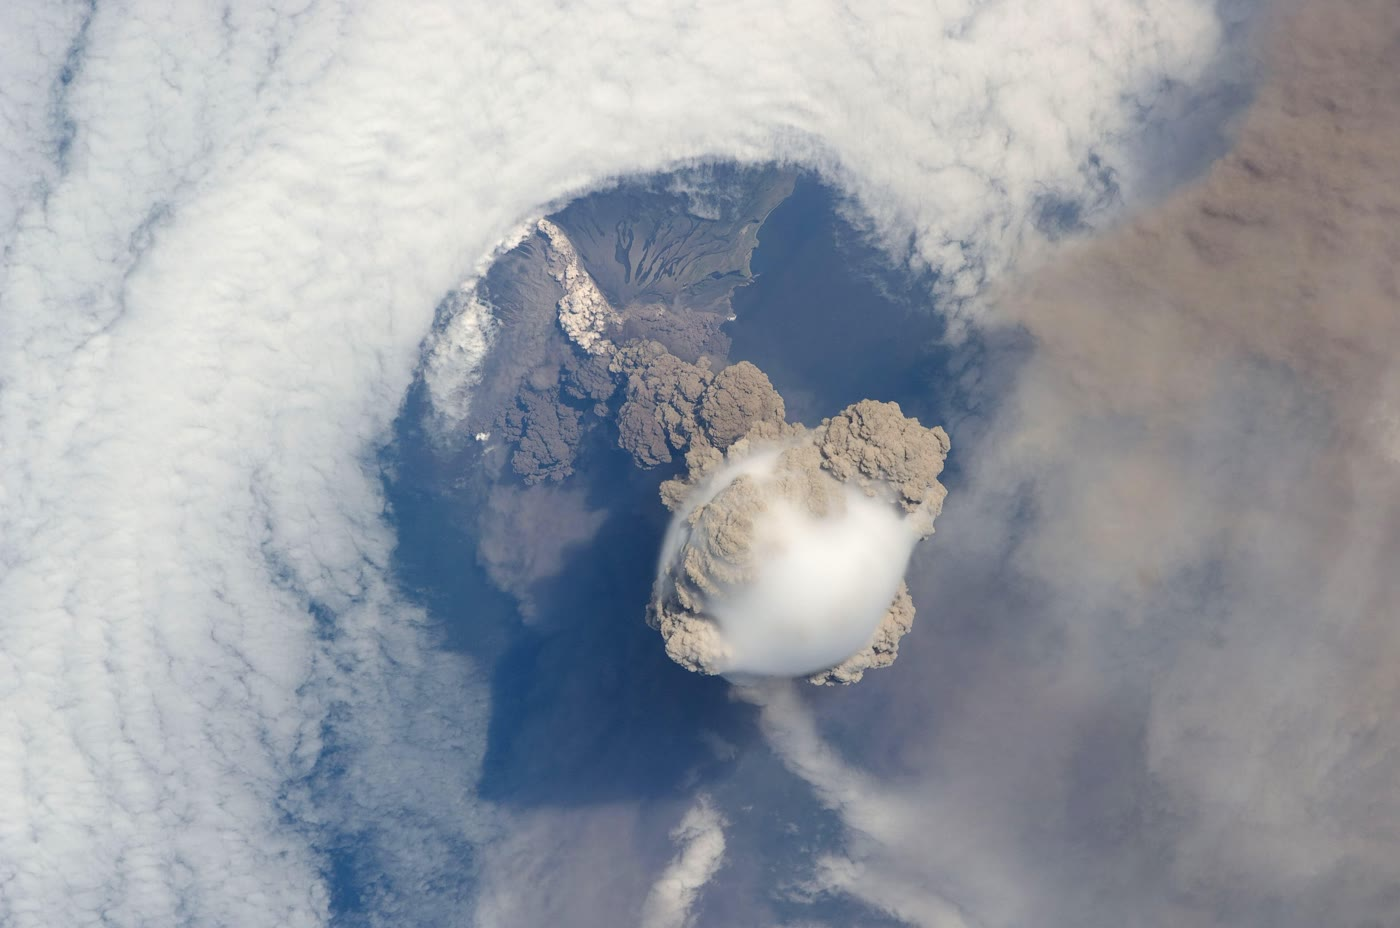
\includegraphics[width=0.66\linewidth]{images/book3/b1-sarychev-iss.jpg}
\par\smallskip{\small Sarychev Peak, un volcán del arco de las Kuriles en la isla de Matua, en una etapa temprana de erupción el 12 de junio de
2009, visto desde la Estación Espacial Internacional a través de un hueco en las nubes. La ceniza gris, probablemente un flujo piroclástico,
desciende de la cumbre, y una capa lisa de nube, un pileo, se asienta sobre la columna ascendente; la ceniza de la erupción se detectó a más de
\qty{2400}{km}. Fotografía: NASA, dominio público (Wikimedia Commons).}
\label{fig:b1:active-margins:sarychev}
\end{omfigure}
% ledger: nasa:sarychev, commons:sarychev

La \omterm{def:b1:layered-earth:layers}{corteza} bajo los arcos se engrosa tanto por acortamiento como por el magma añadido desde abajo; bajo los arcos construidos sobre continentes,
como los Andes, está entre las más gruesas de la Tierra.

Tras algunos arcos la placa cabalgante se separa. Dan Karig explicó estas cuencas marginales del Pacífico occidental dentro de la tectónica de
placas, en 1971: cuando la losa se hunde empinada y retrocede, la fosa y el arco migran hacia la placa que se hunde, y la placa que queda detrás
se estira hasta romperse, dejando a veces un arco remanente extinto al otro lado. En el modelo de placas usado arriba, la expansión de tras-arco
va a unos \qty{32}{mm.yr^{-1}} en la cuenca de las Marianas cerca de \ang{18}\,N, y a más de \qty{110}{mm.yr^{-1}} en el norte de la cuenca de
Lau, detrás de Tonga. Donde la losa es somera, en cambio, arrastra la placa cabalgante, cuya \omterm{def:b1:layered-earth:layers}{corteza} se acorta y engrosa detrás del arco, como
detrás de los Andes.
% ledger: karig:marginal-basins, data:pb2002 (ridge_budget.py: Mariana 32.4, Lau 117.5 mm/yr)

\begin{inthefield}[Alerta de tsunami]
Un centro de alerta de tsunamis dispone de minutos. En 2011 la primera alerta para la costa del noreste de Japón llegó unos tres minutos después
del terremoto, a partir de una magnitud basada en las ondas sísmicas de periodo corto; para terremotos de magnitud 8 o más, esa magnitud se
subestima, y con ella la altura del tsunami. La magnitud de momento, que no se satura, tardó unos quince minutos: los sismómetros de banda
ancha de Japón habían sido llevados más allá de su rango. Desde 2013, cuando el tamaño de un terremoto tan grande es incierto, la primera alerta
supone el terremoto mayor posible allí y describe el tsunami con palabras, como «enorme», en lugar de con un número; y los pronósticos se apoyan
en medidas del mar mismo, mar adentro, con boyas posicionadas por satélite y sensores de presión en el fondo, que ven la ola antes de que llegue
a la costa.
% ledger: jma:warning

\smallskip
\begin{center}
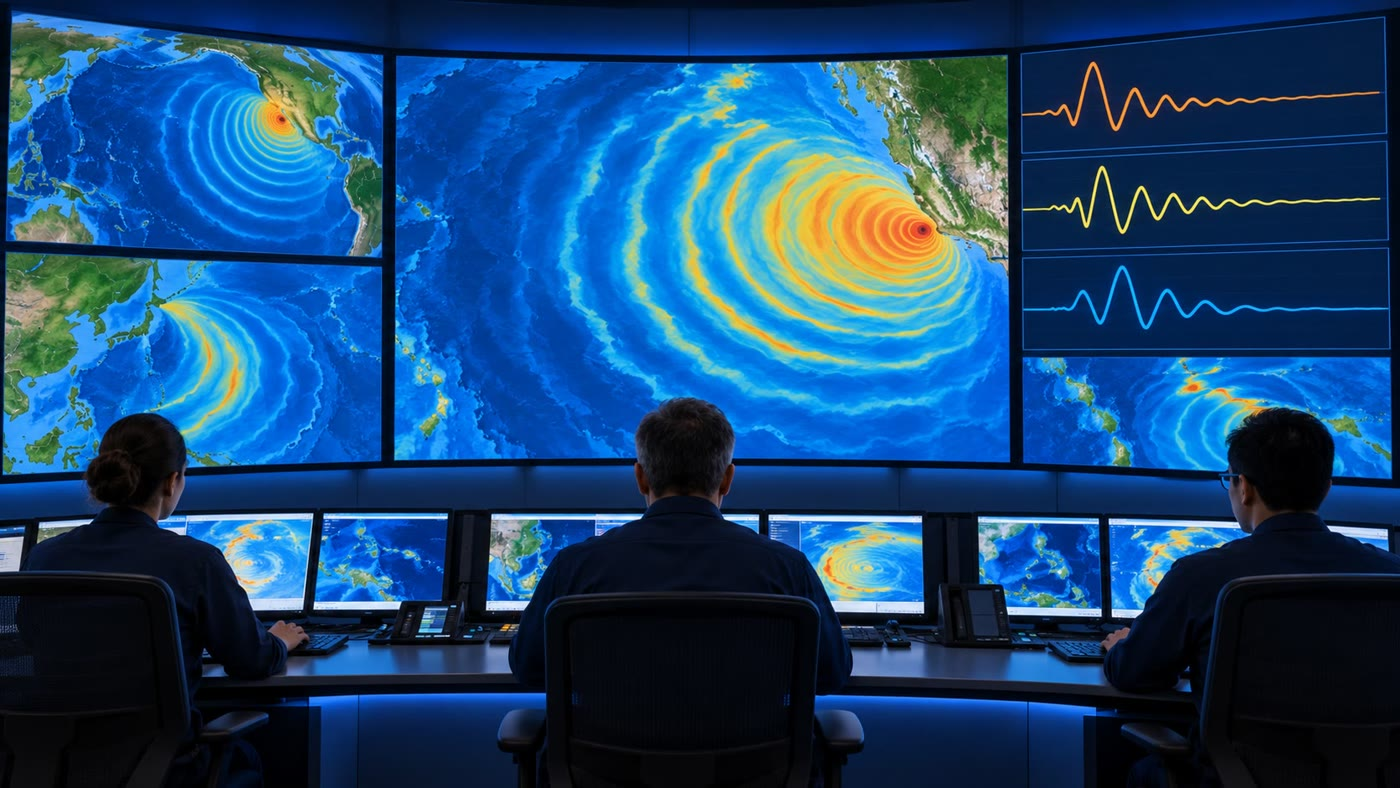
\includegraphics[width=0.7\linewidth]{images/book3/ai/b1-tsunami-centre.jpg}

{\scriptsize Oficiales de guardia en un centro de alerta de tsunamis, ante pantallas de frentes de ola calculados y registros del nivel del mar
(ilustración generada por IA).}
\end{center}
\end{inthefield}

\section{Ejercicios}

\begin{exercise}[$\star$]\label{exo:b1:active-margins:1}
Una fosa yace \qty{3}{km} bajo el fondo oceánico que la rodea. (a) Si no estuviera compensada, ¿en cuánto bajaría la gravedad allí la roca que
falta, de densidad \qty{2700}{kg.m^{-3}}, sustituida por agua de mar de densidad \qty{1000}{kg.m^{-3}}? Úsese la placa de Bouguer, con
$G = \qty{6.674e-11}{m^3.kg^{-1}.s^{-2}}$. (b) Compárese con la anomalía observada sobre la fosa de las Kuriles, unos \qty{-260}{\milli\gal},
donde la fosa yace \qty{3.5}{km} bajo el fondo que la rodea: rehágase el cálculo para esa profundidad.
(c) ¿Por qué el agua de una fosa de solo decenas de kilómetros de anchura da menos que la fórmula de la losa, y dónde debe yacer el resto del déficit?
\end{exercise}

\begin{exercise}[$\star$]\label{exo:b1:active-margins:2}
La placa del Pacífico entra en la fosa de las Kuriles a \qty{82}{mm.yr^{-1}}. (a) ¿Qué longitud de placa se hunde en 10 millones de años? (b) Si la losa
se hundiera a lo largo de una trayectoria recta que buza \ang{45}, ¿a qué profundidad estaría entonces su borde delantero? (c) ¿Cuánto tarda en
alcanzar los \qty{600}{km}?
\end{exercise}

\begin{exercise}[$\star$]\label{exo:b1:active-margins:3}
Los volcanes se alzan sobre el lugar donde una losa recta está a \qty{110}{km} de profundidad. Calcúlese la \omterm{def:b1:active-margins:volcanic-arc}{brecha arco--fosa} para una losa que buza
\ang{30}, \ang{45} y \ang{60}. ¿Qué arco yace más lejos de su fosa?
\end{exercise}

\begin{exercise}[$\star$]\label{exo:b1:active-margins:4}
En el modelo digital de placas del capítulo, unos \qty{2.7}{km^2} de fondo oceánico se hunden cada año por las fronteras de subducción, a lo largo
de unos \qty{51000}{km}, y unos \qty{3.0}{km^2} se forman a lo largo de unos \qty{67000}{km} de dorsales de expansión.
(a) Calcúlense la velocidad media de convergencia y la velocidad media total de expansión, en \unit{mm.yr^{-1}}. (b) En el conjunto de sus fronteras
el modelo destruye tanta área como forma. ¿Adónde va el resto del fondo nuevo?
% ledger: data:pb2002 (ridge_budget.py: 2.739 km2 over 51471 km; 3.009 km2 over 67340 km; all 3.511 vs 3.519)
\end{exercise}

\begin{exercise}[$\star\star$]\label{exo:b1:active-margins:5}
Cuatro terremotos de una sección yacen en $(x, z) = (200, 150)$, $(300, 250)$, $(400, 330)$ y $(500, 430)$, en kilómetros. (a) Ajústese la recta de la
losa por mínimos cuadrados y dése su \omterm{def:b1:geological-maps:attitude}{buzamiento}. (b) ¿Dónde alcanza la recta la superficie? (c) Compárese con el \omterm{def:b1:geological-maps:attitude}{buzamiento} de la recta que pasa solo
por el primero y el último terremoto.
\end{exercise}

\begin{exercise}[$\star\star$]\label{exo:b1:active-margins:6}
Una losa modelo buza \ang{25} desde la fosa hasta \qty{50}{km}, y luego \ang{45}. El frente volcánico se alza donde la losa está a \qty{110}{km} de
profundidad. (a) Calcúlese la \omterm{def:b1:active-margins:volcanic-arc}{brecha arco--fosa}. (b) Compárese con una losa que buza \ang{45} en todo su recorrido. (c) El segmento profundo,
prolongado hacia arriba, alcanza la superficie: ¿dónde? Compárese con la recta de las Kuriles, que la alcanza \qty{53}{km} hacia tierra desde la fosa.
(d) ¿Qué brecha daría un segmento profundo de \ang{60}?
\end{exercise}

\begin{exercise}[$\star\star$]\label{exo:b1:active-margins:7}
(a) Según la proposición de la cáscara curvada, ¿qué radio angular, y qué radio en kilómetros ($R = \qty{6371}{km}$), debe tener un arco sobre una
losa que buza \ang{45}? ¿\ang{30}? ¿\ang{70}? (b) ¿Qué arcos están más estrechamente curvados? (c) La losa de las Kuriles buza \ang{44.9} y la fosa de
las Kuriles se ajusta a un círculo de \ang{21.9}: calcúlese la diferencia relativa respecto de la predicción.
\end{exercise}

\begin{exercise}[$\star\star$]\label{exo:b1:active-margins:8}
Tómese una conductividad de \qty{2.5}{W.m^{-1}.K^{-1}} y una temperatura en superficie de \qty{10}{\celsius}. (a) Calcúlese el gradiente de temperatura en
superficie bajo un \omterm{def:b1:active-margins:active-margin}{antearco} que pierde \qty{35}{mW.m^{-2}} y bajo un tras-arco que pierde \qty{80}{mW.m^{-2}}. (b) Extrapolando linealmente estos gradientes,
estímese la temperatura a \qty{30}{km} en cada uno. (c) Los \omterm{def:b1:layered-earth:discontinuity}{Moho} de tras-arco se miden a 800 a \qty{900}{\celsius}. ¿Por qué la estimación lineal es demasiado alta?
% ledger: hyndman:backarc (back-arc 70-85, Moho 800-900); the forearc value is an exercise value
\end{exercise}

\begin{exercise}[$\star\star$]\label{exo:b1:active-margins:9}
En el modelo de placas del capítulo, la cuenca de las Marianas se abre cerca de \ang{18}\,N a una velocidad total de unos \qty{32}{mm.yr^{-1}}. (a) Exprésese esta
velocidad en \unit{km.Myr^{-1}}, y dése la velocidad media de cada flanco si la expansión es simétrica. (b) ¿Cuánto tardaría la cuenca en abrirse \qty{100}{km}
a esta velocidad? (c) Dense dos razones por las que la edad de una \omterm{def:b1:active-margins:active-margin}{cuenca de tras-arco} no puede leerse simplemente a partir de su anchura y de su velocidad actual.
% ledger: data:pb2002 (ridge_budget.py: mariana_18n_mm_yr 32.4)
\end{exercise}

\begin{exercise}[$\star\star\star$]\label{exo:b1:active-margins:10}
Una losa de \qty{100}{km} de espesor se hunde a \qty{82}{mm.yr^{-1}} a lo largo de una trayectoria que buza \ang{45}. Tómese $\kappa = \qty{e-6}{m^2.s^{-1}}$. (a) ¿Cuánto tarda en alcanzar
los \qty{600}{km}? (b) ¿Hasta dónde se difunde el calor en ese tiempo, por $\sqrt{\kappa t}$? (c) ¿Cuánto tardaría el calor en llegar a su centro? (d)
Concluya sobre la temperatura de la losa a \qty{600}{km} y sobre sus terremotos.
\end{exercise}

\begin{exercise}[$\star\star\star$]\label{exo:b1:active-margins:11}
Un \omterm{def:b1:active-margins:accretionary}{prisma de acreción} modelo tiene sección triangular: su superficie inclina $\alpha = \ang{4}$ hacia la fosa y su base buza $\beta = \ang{6}$ bajo él, ambas
se encuentran en su pie; mantiene estos ángulos al crecer. (a) Muéstrese que su área es $A = \frac12 L^2(\tan\alpha + \tan\beta)$ para una anchura $L$, cuando los
ángulos son lo bastante pequeños para que la altura en la parte posterior sea $L(\tan\alpha + \tan\beta)$. (b) Llega a una placa convergente a \qty{40}{mm.yr^{-1}} una
capa de sedimento de \qty{1}{km} de espesor, y todo se acreciona: calcúlese la anchura tras 1, 4 y 10 millones de años. ¿Cómo crece $L$ con el tiempo? (c) ¿Qué pasa si
la mitad del sedimento se hunde con la losa?
\end{exercise}

\begin{exercise}[$\star\star\star$]\label{exo:b1:active-margins:12}
(a) Muéstrese que la recta de mínimos cuadrados pasa por el punto medio $(\bar x, \bar z)$. (b) Un catálogo enumera cada profundidad \qty{10}{km} demasiado profunda.
¿Cómo cambian la pendiente y la ordenada en el origen de la recta ajustada? (c) Las distancias $x$ se miden todas desde un punto de la fosa situado \qty{20}{km} demasiado
hacia tierra, de modo que cada $x$ es \qty{20}{km} demasiado pequeña. ¿Cómo cambian la pendiente y la ordenada en el origen? (d) ¿Cambia alguno de estos errores el \omterm{def:b1:geological-maps:attitude}{buzamiento}?
\end{exercise}

\section{Problema: Leer una zona de subducción a partir de sus terremotos}

\begin{problem}[{Problema de fin de semana --- la losa de las Kuriles a partir de ocho terremotos, a qué velocidad se hunde, lo que dicen su gravedad
y su flujo de calor, y dónde deben situarse sus volcanes}]
\label{pb:b1:active-margins:1}
% values: calc/ch14.py; the eight events are real (USGS catalogue, rounded to the km)
% from figdata/out/bachelor-1-slab_seismicity-section.dat
% ledger: data:b3-usgs-kuril, data:pb2002, data:b2-seafloor-age, syracuse:arc-depth, frank:arcs,
% data:b3-grav-kuril, parsons:plate-model, hyndman:backarc; the forearc heat flow is an exercise value
Ocho terremotos de la losa de las Kuriles, todos más profundos que \qty{70}{km}, se enumeran según su distancia $x$ a la fosa a lo largo de la
línea de sección, hacia el mar de Ojotsk, y su profundidad $z$, ambas redondeadas al kilómetro.

\begin{center}
\small
\begin{tabular}{lcccccccc}
\hline
terremoto & 1 & 2 & 3 & 4 & 5 & 6 & 7 & 8\\
$x$ (\unit{km}) & 155 & 222 & 305 & 319 & 431 & 533 & 578 & 609\\
$z$ (\unit{km}) & 96 & 169 & 245 & 272 & 389 & 489 & 518 & 573\\
magnitud & 5.5 & 5.1 & 5.0 & 5.4 & 5.3 & 5.3 & 5.2 & 6.4\\
\hline
\end{tabular}
\end{center}

\medskip
\noindent\textbf{Parte I --- La recta de la losa.}
\begin{enumerate}
  \item Represéntense los ocho terremotos a la misma escala en ambos ejes, con la profundidad hacia abajo.
  \item Calcúlense $\sum x_i$, $\sum z_i$, $\sum x_i^2$, $\sum x_i z_i$ y las medias $\bar x$ y $\bar z$.
  \item Calcúlense $S_{xx}$ y $S_{xz}$, y luego la pendiente de la recta de mínimos cuadrados con tres decimales y su ordenada en el origen con un decimal.
  \item ¿Cuál es el \omterm{def:b1:geological-maps:attitude}{buzamiento} de la losa?
  \item ¿Dónde alcanza la recta la superficie? ¿Qué dice esto de la forma de la losa cerca de la fosa?
  \item Calcúlese el desajuste $z_i - (a + s x_i)$ de cada terremoto. ¿Cuáles yacen más lejos de la recta, y cuánto?
\end{enumerate}

\medskip
\noindent\textbf{Parte II --- Con qué velocidad se hunde la losa.} Al principio de la sección el modelo PB2002 da una convergencia de
\qty{87.4}{mm.yr^{-1}}: respecto de la placa de Ojotsk, la placa del Pacífico se mueve hacia el \omterm{def:b1:spherical-astronomy:horizontal}{acimut} \ang{300}. La línea de sección,
perpendicular a la fosa, corre hacia el \omterm{def:b1:spherical-astronomy:horizontal}{acimut} \ang{320.9}.
\begin{enumerate}[resume]
  \item Calcúlese el ángulo entre la convergencia y la línea de sección, y luego las componentes de la convergencia perpendicular y paralela a la fosa.
  \item ¿Qué longitud de placa se hunde en la fosa en 10 millones de años?
  \item Usando el \omterm{def:b1:geological-maps:attitude}{buzamiento} de la pregunta 4 (redondeado a \ang{45}), ¿cuánto tarda la losa en llevar un punto de su cima desde la fosa hasta el
        terremoto más profundo de la franja, a \qty{632}{km}? Despréciese el \omterm{def:b1:geological-maps:attitude}{buzamiento} más suave cerca de la fosa.
  \item La placa tiene unos \qty{122}{Myr} en la fosa. ¿Qué edad tiene el fondo marino que está ahora a \qty{632}{km} de profundidad?
  \item Según $\sqrt{\kappa t}$, con $\kappa = \qty{e-6}{m^2.s^{-1}}$, ¿hasta dónde se ha difundido el calor en la losa durante ese descenso? Compárese
        con su espesor, unos \qty{100}{km}.
\end{enumerate}

\medskip
\noindent\textbf{Parte III --- Gravedad y flujo de calor.} Tómese una conductividad de
\qty{2.5}{W.m^{-1}.K^{-1}}.
\begin{enumerate}[resume]
  \item El fondo oceánico antiguo frente a la fosa pierde unos \qty{43}{mW.m^{-2}}, el tras-arco unos \qty{80}{mW.m^{-2}}; tómense
        \qty{35}{mW.m^{-2}} para el \omterm{def:b1:active-margins:active-margin}{antearco}. Calcúlese el gradiente de temperatura cerca de la superficie de cada uno.
  \item Explíquese por qué el \omterm{def:b1:active-margins:active-margin}{antearco} pierde menos calor que el fondo oceánico antiguo que tiene delante.
  \item La \omterm{def:b1:isostasy-gravity:anomalies}{anomalía de aire libre} sobre la fosa de las Kuriles es de unos \qty{-260}{\milli\gal}. ¿Qué espesor de roca, \qty{1700}{kg.m^{-3}} más
        densa que el agua, necesitaría una placa de Bouguer para dar este déficit? Compárese con la profundidad de la fosa bajo el fondo que la
        rodea, unos \qty{3.5}{km}.
  \item Supóngase ahora que toda la placa se empuja hacia abajo \qty{3.5}{km}: el agua ocupa el lugar de la roca en su parte superior, y su \omterm{def:b1:layered-earth:layers}{corteza}
        el lugar del \omterm{def:b1:layered-earth:layers}{manto} en su base, de modo que en total el \omterm{def:b1:layered-earth:layers}{manto} de densidad \qty{3300}{kg.m^{-3}} se sustituye por agua. Calcúlese la anomalía de la
        placa de Bouguer. ¿Por qué la fosa real, de solo decenas de kilómetros de anchura, da menos?
  \item La fosa y la elevación exterior no están en equilibrio isostático. ¿Qué las mantiene fuera de él?
\end{enumerate}

\medskip
\noindent\textbf{Parte IV --- Dónde deben estar los volcanes.} Úsese la recta de la pregunta 3, con su pendiente y su ordenada redondeadas.
\begin{enumerate}[resume]
  \item El primer volcán de la franja está a \qty{164}{km} de la fosa. ¿Qué profundidad tiene la losa bajo él?
  \item ¿Está esta profundidad dentro del rango encontrado bajo los arcos, de 72 a \qty{173}{km}? ¿A qué distancia está del promedio, \qty{105}{km}?
  \item ¿A qué distancia de la fosa la losa está a \qty{100}{km} de profundidad?
  \item Según la proposición de la cáscara curvada, ¿qué radio angular debe tener el arco de las Kuriles, y qué radio en kilómetros?
  \item La fosa de las Kuriles se ajusta a un \omterm{def:b1:spherical-astronomy:spherical-triangle}{círculo menor} de \ang{21.9}. Compárese.
  \item Los volcanes de arco se alzan, en promedio, donde la losa está a unos \qty{105}{km} de profundidad. ¿A qué distancia de la fosa alcanza la
        recta de la losa esa profundidad?
  \item Compárese esta distancia con los \qty{164}{km} observados: ¿en cuántos kilómetros y en qué fracción difiere?
  \item Al kilómetro más próximo, ¿qué \omterm{def:b1:active-margins:volcanic-arc}{brecha arco--fosa} predice la recta de la losa de las Kuriles para volcanes que se alzan sobre la losa a \qty{105}{km}?
\end{enumerate}
\end{problem}
